\documentclass[danish]{article}
\usepackage[utf8]{inputenc}
\usepackage[danish]{babel}
\usepackage[T1]{fontenc}	
\usepackage[a4paper, , margin=1in]{geometry}

\usepackage[version=3]{mhchem} % Package for chemical equation typesetting
\usepackage{siunitx} % Provides the \SI{}{} and \si{} command for typesetting SI units
\usepackage{graphicx} % Required for the inclusion of images
\usepackage{subcaption} % Add the possibility for subfigures/subcaptions.
\usepackage{natbib} % Required to change bibliography style to APA
\usepackage{amsmath} % Required for some math elements

\usepackage{float}
\graphicspath{ {graphics/} }

\setlength\parindent{0pt} % Removes all indentation from paragraphs

\renewcommand{\labelenumi}{\alph{enumi}.} % Make numbering in the enumerate environment by letter rather than number (e.g. section 6)
\begin{document}

\title{\textbf{Analog System Design} \\Eksamensforberedelse}
\author{Jonas Lind}
\date{14-08-2017}
\maketitle
\section{Effektforstærkerøvelse: DC}
\begin{itemize}
	\item Klasse AB \SI{30}{\watt} forstærker til \SI{8}{\ohm} højtaler.
	\item Indgangsignalet har signalamplitude på 1V.
\end{itemize}

\paragraph{Spændingsvinget} som er nødvendigt for at drive højtaleren ved \SI{30}{\watt} beregnes til \SI{22}{\volt}. Der skal være plads til to basis-emitter strækninger for udgangstrinnet, noget lignende til den øvrige elektronik og ripple i effektforsyningen og  \SI{10}{percent}  på netspændingen så effektforsyningen bør placeres cirka \SI{5}{\volt} højere end kravet til $V_O$ og det giver værdien til $+-\SI{27}{\volt}$.

\begin{equation}
P_O = \dfrac{V_{RMS}}{R_L}
\end{equation}

\begin{equation}
V_{RMS} = \sqrt{P_O R_L} = \SI{15.5}{\volt}
\end{equation}

\begin{equation}
V_O = V_{RMS} \sqrt{2} = \SI{22}{\volt}
\end{equation}

\paragraph{Strømsvinget} som er nødvendigt på forstærkerens udgang igennem de \SI{8}{\ohm} findes til at være \SI{3.65}{\ampere}, ved en nominel modstandsværdi på \SI{6}{\ohm}. Dette er gældende da højttalerens svingspole har en DC modstand $R_{DC}$ på typisk \SI{80}{\percent}  af den nominelle værdi. Der forventes en middelstrøm fra effektforsyningen på $I_{DC} = \SI{1.16}{\ampere}$.

\begin{equation}
I_{O\,PEAK} = \dfrac{V_O}{R_L} = \SI{3.65}{\ampere}
\end{equation}

\begin{equation}
I_{DC} = \dfrac{I_{O\,PEAK}}{\pi} = \SI{1.16}{\ampere}
\end{equation}

\paragraph{Udgangstrinnet} benytter et darlington par af to emitter følgere (common collector) for at øge strømforstærkningen. Drivertrinnet skal levere basisstrømmen til udgangstransistorerne 2N3055 og MJ2955 og med $\beta_{10} = \beta_{11} = 20$ som strømforstærkning i $T_{10}$ og $T_{11}$ behøves en strøm på \SI{183}{\milli\ampere}.

\begin{equation}
I_B = \dfrac{I_{O\,PEAK}}{\beta} = \SI{183}{\milli\ampere}
\end{equation}

Basisstrømmen til drivertrinnet er \SI{5}{\milli\ampere} ved en strømforstærkning på $\beta_8 = \beta_9 = 40$.

\begin{equation}
I_B = \dfrac{\SI{183}{\milli\ampere}}{\beta} = \SI{4.58}{\milli\ampere}
\end{equation}

Den samlede strømforstærkning er 800 og forstærker basisstrømmen til drivertrinnet på \SI{4.58}{\milli\ampere} op til det nødvendige strømsving i udgangen på \SI{3.65}{\ampere}.

\begin{equation}
\beta = \beta_1 \beta_2 = 20 {\cdot} 40 = 800
\end{equation}

Dette sænker de \SI{3.65}{\ampere} udganstrinnet skal levere til \SI{4.58}{\milli\ampere}.Således belaster udgangstrinnet VAS-trinnet minimalt.
En strømkilde leverer basestrømmen på \SI{4.66}{\milli\ampere}.


\paragraph{Diode biasing} benyttes for at minimere crossover distortion. Fire dioder sættes i serie for at skabe et fast spændingsfald på \SI{2.8}{\volt} mellem de to transistores baser. 

\paragraph{Strømkilde}
Strømkilden sørger for at der løber en strøm i dioderne, der giver et konstant spændingsfald. Der anvendes en strømkilde istedet for en modstand, da der vil blive afsat for meget effekt i denne.
Modstanden $R_E (R_{7})$ styrer strømmen $I_O = \SI{4.66}{\milli\ampere}$. 

\begin{figure} [H]
	\centering
	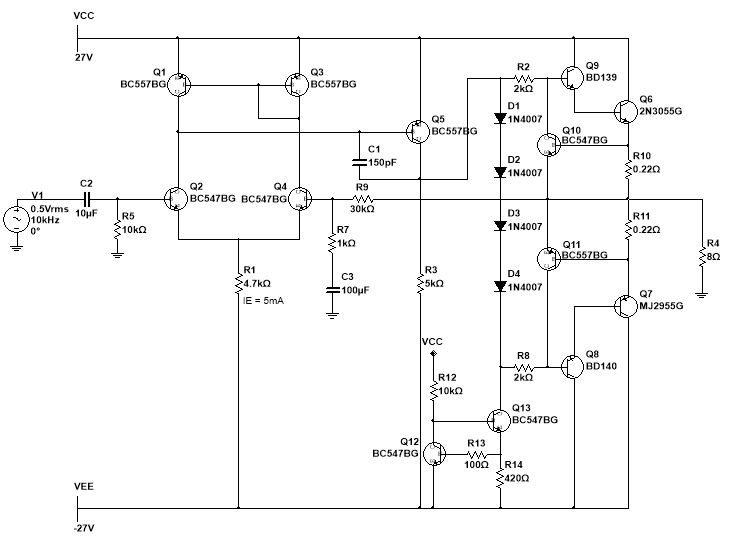
\includegraphics[width=\linewidth]{graphics/PowerAmp_schematic}
	\caption{Kredsløbsdiagram for effektforstærker klasse AB.}
	\label{fig:PowerAmp_schematic}
\end{figure}

\newpage
\section{Effektforstærkerøvelse: AC}

\subsection{Forstærkning og stabilitet}
\begin{itemize}
	\item Der laves en dominerende pol for at sikre stabilitet ved at forstærkningen er sænket til under 1 når fasedrejet er 180°.
	\item Dette begrænser forstærkerens båndbredde.
	\item Slew rate begrænsning af kondensatoren $C_C$ og strømmen $I_E$.
	\item Ved hurtig og stor udstyring bliver sinusen til en trekant pga den begrænsede hastighed.
\end{itemize}

\paragraph{Åben-sløjfe forstærkningen} benytter en transistors strømforstærkning $\beta$ for T5 til at forstærke differentialtrinnets udgangsstrøm. Denne strøm bliver ledet gennem modstanden $R_C$, som laver det om til en strøm. 
Indgangsmodstanden for en emitterfølger er belastningen $R_L$ gange med den samlede strømforstærkning til $R_C = \SI{4.8}{\kilo\ohm}$.

\begin{equation}
R_C = \beta_8 \beta_{10} R_L = \SI{4.8}{\kilo\ohm}
\end{equation}

DC forstærkningen beregnes herefter til $A_{DC} = 194000$ ved en belastning på $R_L = \SI{6}{\ohm}$.

\begin{equation}
A_{DC} = g_m \beta_5 R_C = 194000
\end{equation}

I en integreret forstærker benyttes ofte flere transistorer til at forøge den resulterende strømforstærkning mens en effektforstærker som oftest nøjes med en enkelt transistor da der ikke er behov for den ekstremt høje forstærkning ved DC. 

\paragraph{Kompenseringskondensatoren} skal sikre stabilitet ved at reducere forstærkningen til en ved den laveste af de høje poler der antages givet af $R_C$ og $C_{\si{\micro}}$ for T5, T8 og T9 i parallel.
Ved en værdi på \SI{10}{\pico\farad} findes $f_H = \SI{3.3}{\mega\hertz}$ og den dominerende pol $f_0$ findes til \SI{17}{\hertz}. 

\begin{equation} 
f_H  = \frac{1}{2\pi R_C C_{\si{\micro}}} = \SI{3.3}{\mega\hertz}
\end{equation}

\begin{equation}
f_0 = \frac{f_H}{A_{DC}} = \SI{17}{\hertz}
\end{equation}

Ved den aktuelle forstærkning på $A_{CL} = 31$ kan den dominerende pol $f_P$ findes til \SI{530}{\hertz} som er tilstrækkelig for stabilitet.

\begin{equation}
f_P = A_{CL} f_0 = \SI{530}{\hertz}
\end{equation}

Den dominerende pol $f_0$ ligger så lavt at systemet bliver ubetinget stabilt.

\begin{equation} 
f_0  \leq \frac{f_h A_{CL}}{4\,A_{DC}} = \SI{133}{\hertz}
\end{equation}

Kompenseringskondensatoren kan herved findes.

\begin{equation} 
C_C  = \frac{1}{2\pi \beta f_0 R_C}
\end{equation}

\begin{figure} [H]
	\centering
	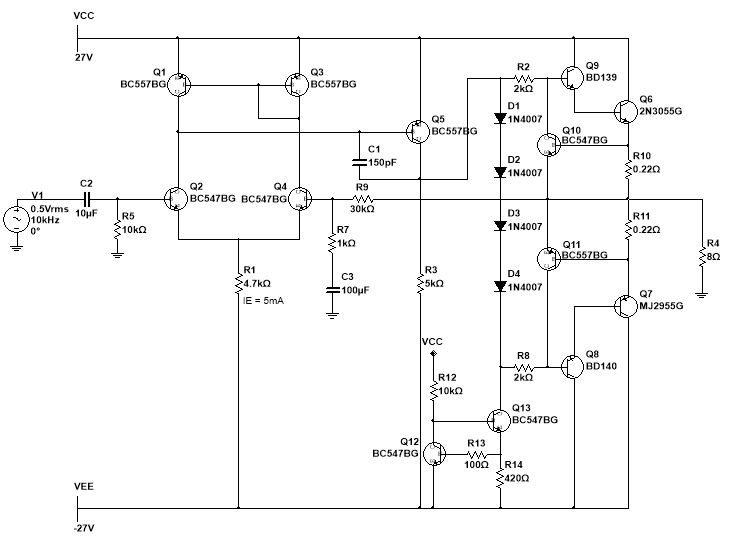
\includegraphics[width=\linewidth]{graphics/PowerAmp_schematic}
	\caption{Kredsløbsdiagram for effektforstærker klasse AB.}
	\label{fig:PowerAmp_schematic1}
\end{figure}

DC forstærkningen er således givet ved:
\begin{equation} 
A_{DC} = g_m \beta R_C
\end{equation}

Transkonduktansen gm i differentialtrinnet T1 ... T4 beregnes til 0,1 

Kondensatoren $C_C$ skaber en dominerende pol ved $f_0$, som sikrer stabilitet.

\begin{equation} 
f_0 = \dfrac{1}{2 \pi \beta R_C C_C}
\end{equation}

Slew-raten (SR) begrænses af kondensatoren og strømmen $I_E$.

\begin{equation} 
SR = \dfrac{I_E}{C_C}
\end{equation}

\begin{figure} [H]
	\centering
	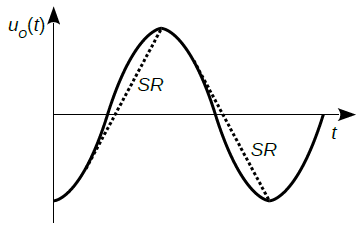
\includegraphics[width=0.4\linewidth]{graphics/slewrate}
	\caption{Operationsforstærkerens slew rate.}
	\label{fig:slewrate}
\end{figure}

Den dominerende pol giver stabilitet, men begrænser også hvor hurtigt udgangen kan flyttes. Hvis værdien forsøges overskredet bliver signalet forvrænget.

\subsection{Transistor - AC model}
\subsection{Diode - AC model}

\newpage
\section{Effektforstærkerøvelse: Effektafsættelse}
\subsection{Beregning af effektafsættelse}
Herunder regnes den totale effekt afsat i forstærkeren og ud fra den findes effekten afsat i udgangstrinnet.\\

Den tilførte effekt på \SI{67}{\watt} ved \SI{30}{\watt} afgivet i nominelt \SI{8}{\ohm}. 

\begin{equation}
I_{O\,PEAK} = \SI{3.65}{\ampere}
\end{equation}

\begin{equation}
I_{DC} = \dfrac{I_{O\,PEAK}}{\pi} =\SI{1.16}{\ampere}
\end{equation}

\begin{equation}
P_{CC} = U_{CC}(I_{PEAK}-I_{DC})=\SI{67.2}{\watt}
\end{equation}

Effekttabet i udgangstransistorerne T9 og T10 bliver \SI{32}{\watt} samlet og derfor forventes et tab på \SI{16}{\watt} i hver transistor. 

\begin{equation}
P_O = \dfrac{U_{CC}U_O}{\pi R_L} =\SI{31.2}{\watt}
\end{equation}

\subsection{SOA}
SOA er en betegnelse for safe-operating area.
SOA findes ved at kombinere følgende tre begrænsninger:
\begin{itemize}
	\item $I_{C,MAX}$
	\item  $U_{CE,MAX}$
	\item  $P_{MAX}$
\end{itemize}

$P_{MAX}$ giver skæringspunkterne for 2N3055:

\begin{equation}
I_C = \dfrac{P_{MAX}}{U_{CE}} = \dfrac{\SI{115}{\watt}}{\SI{60}{\volt}} = \SI{1.9}{\ampere}
\end{equation}

\begin{equation}
U_{CE} = \dfrac{P_{MAX}}{I_C} = \dfrac{\SI{115}{\watt}}{\SI{15}{\ampere}} = \SI{7.7}{\volt}
\end{equation}

\begin{figure} [H]
	\centering
	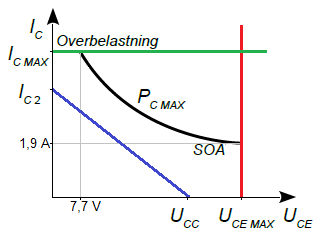
\includegraphics[width=0.4\linewidth]{graphics/soa}
	\caption{Safe-operating area.}
	\label{fig:soa}
\end{figure}


\subsection{Termisk modstand}
En køleprofil beskrives normalt ved en termisk modstand og Ohms lov antages at gælde for det termiske system. 
Man siger at effektstrømmen $P$ løber gennem den termiske modstand $R_{th}$ og det danner et temperaturfald på $R_{th}P$ som hæver temperaturen $T$ over omgivelsestemperaturen $T_{amb}$.
Den termiske modstand kaldes undertiden for køleprofilets K-værdi og enheden er en stigning i temperatur per effekt.

\begin{equation}
T = (R_{th} P + T_{amb}
\end{equation}

\begin{itemize}
	\item Angiver evnen til at transportere og afsætte varme, f.eks. fra transistorens junction til dens overflade.
	\item Måles i \SIUnitSymbolCelsius /\si{\watt}
	\item Jo højere værdi, jo varmere vil et komponent blive ved en given afsat effekt.
\end{itemize}

\begin{figure} [H]
	\centering
	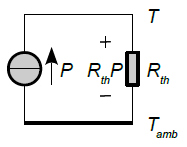
\includegraphics[width=0.3\linewidth]{graphics/ohmslovanalogi}
	\caption{Beregning af temperaturstigning ved en effektstrøm P i en termisk modstand.}
	\label{fig:ohmslovanalogi}
\end{figure}

\begin{itemize}
	\item $R_{th\:j-mb}$
	\begin{itemize}
		\item Den termiske modstand fra PN overgangen \textit{(junction)} til monteringsflade	\textit{(mounting base)}.
	\end{itemize}
	\item $R_{th\: mb-hs}$
	\begin{itemize}
		\item Den termiske modstand mellem monteringsflade	\textit{(mounting base)} og køleprofilet \textit{(heat sink)}.
		\item Inkluderes i den termiske model når det er nødvendigt at isolere transistoren fra køleprofilet med en isolationsskive af glimmer eller silicone.
	\end{itemize} 
	\item $R_{th\: hs}$ 
	\begin{itemize}
		\item Den eksterne termiske modstand for køleprofilet \textit{(heat sink)}.
	\end{itemize}
\end{itemize}

\begin{equation}
T_j = (R_{th\:j-mb} + R_{th\: mb-hs} + R_{th\: hs})P + T_{amb}
\end{equation}

\begin{figure} [H]
	\centering
	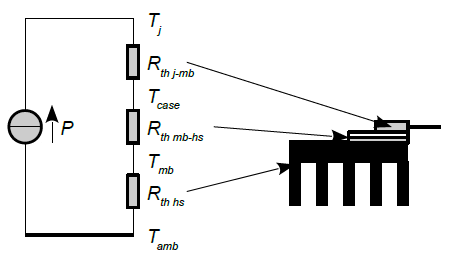
\includegraphics[width=0.5\linewidth]{graphics/termiskdesign}
	\caption{Termisk kredsløb.}
	\label{fig:termiskdesign}
\end{figure}

\subsection{Dimensionering af køling}
Klasse AB forstærkerens effekttransistor junction ønskes kølet til maksimalt \SI{100}{\degreeCelsius}
Ifølge databladet for 2N3055 er junction to case = \SI{1.52}{\degreeCelsius\per\watt}.

\begin{equation}
T_j = (R_{th\:j-mb} + R_{th\: mb-hs} + R_{th\: hs})P + T_{amb}
\end{equation}

\begin{equation}
R_{th\: hs} = \dfrac{T_j-T_{amb}}{P}-R_{th\:j-mb} + R_{th\: mb-hs}
\end{equation}

\begin{equation}
R_{th\: hs} = \dfrac{\SI{100}{\degreeCelsius}-\SI{25}{\degreeCelsius}}{\SI{11}{\watt}}-\SI{1.52}{\degreeCelsius\per\watt} = \SI{5.3}{\degreeCelsius\per\watt}
\end{equation}




\newpage
\section{Effektforstærkerøvelse: Effektforsyning}

\subsection{Transformer}
\begin{itemize}
	\item En transformer kan regulere AC-spændinger (ikke DC!) op og ned.
	\item Lavere antal sekundær vindinger, giver en lavere udgangsspænding.
	\item Varmetab i spolerne \approx \SI{5}{percent}.
\end{itemize}


\subsection{Ensretning}
\begin{itemize}
	\item Full bridge brokoblingen ensretter de positive og negative halvbølger.
	\item Der er to diode-spændingsfald, som sænker spændingen \approx \SI{-1.4}{\volt}.
\end{itemize}

\begin{figure} [H]
	\centering
	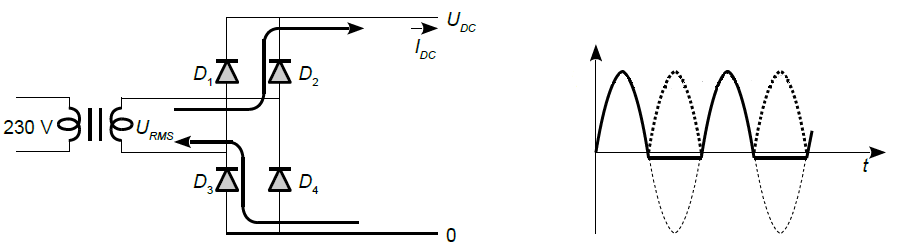
\includegraphics[width=\linewidth]{graphics/ensretning}
	\caption{Helbølgeensretter med brokobling.}
	\label{fig:ensretter}
\end{figure}

\subsection{Udglatning}
\begin{itemize}
	\item Kondensatoren $C_{filter}$ udglatter den ensrettede spænding.
	\item Der vil være ripple, $U_{RIP}$, som øges ved større $I_O$.
	\item $U_{RIP}$ sænkes ved større kondensator.
	\item Elektrolyt-kodensator benyttes.
\end{itemize}

\begin{figure} [H]
	\centering
	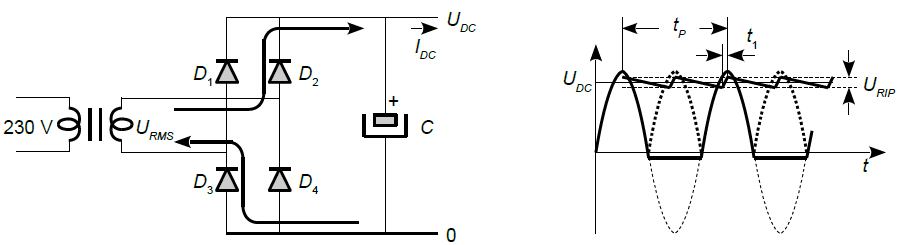
\includegraphics[width=\linewidth]{graphics/udglatning}
	\caption{Udglatning af den ensrettede spænding med kondensator.}
	\label{fig:udglatning}
\end{figure}


\begin{equation}
t_p = \dfrac{1}{\SI{50}{\hertz}} = \SI{20}{\milli\second}
\end{equation}

\begin{equation}
C_{Filter} = \dfrac{I_{DC}t_p}{2 U_{RIP}}
\end{equation}

\begin{itemize}
	\item 2 tallet skyldes at der regnes for en halvperiode $t_p/2$.
\end{itemize}

\newpage
\subsection{Serie regulator}
\begin{itemize}
	\item Lineær spændingsregulator, som afsætter overskydende spænding som varme.
	\item Input kondensatoren sikrer stabilitet, hvis dens forsyning er langt fra input.
	\item Output kodensatoren giver også stabilitet og evnen til hurtigt at levere strøm.
	\item Reguleres internt ud fra en bandgap spændingsreference, $V_{ref}$.
\end{itemize}

\begin{figure} [H]
	\centering
	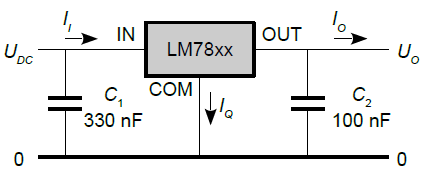
\includegraphics[width=0.6\linewidth]{graphics/serieregulator}
	\caption{Lineær spændingsregulator med afkoblingskondensatorer.}
	\label{fig:serieregulator}
\end{figure}

\begin{equation}
P_{tab} = (U_{DC} - U_O) I_O
\end{equation}

\subsection{DC-DC konverter}
DC konverteren benytter en spole til at optage energi fra indgangen i et kort tidsrum hvorefter energien overføres til udgangen i det efterfølgende tidsrum. 
Den proces gentages i en evindelighed styret af en transistor og en diode der arbejder som kontakter. 
Transistoren kan være bipolar eller felteffekt.
\begin{itemize}
	\item Kan regulere DC spændinger op og ned mere effektivt end lineære regulatorer.
	\item Har en virkningsgrad på over \SI{90}{\percent}.
	\item Der er højfrekvent switching støj på udgangen, hvilket kan være uønsket.
\end{itemize}

\paragraph{Opkonvertering}
\begin{itemize}
	\item Et PWM signal med en frekvens > 100 kHz styrer MOSFET’en.
	\item Når MOSFET'en er tændt løber der en strøm igennem spolen, som oplades. C2 aflades. 
	\item Når MOSFET'en er slukket aflades spolen, som skaber en spænding i serie med $U_{DC}$, som lader C2 op igennem dioden.
	\item Dioden sørger for at kondensatoren ikke aflades tilbage igennem MOSFET’en.
	\item Gøres det hurtigt nok vil $U_O$ altid holdes over $U_{DC}.$
\end{itemize}

\begin{figure} [H]
	\centering
	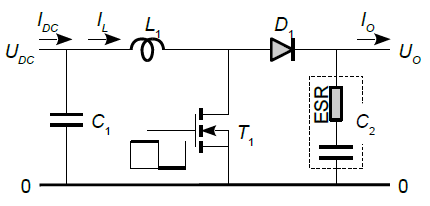
\includegraphics[width=0.6\linewidth]{graphics/opkonvertering}
	\caption{Opkonvetering.}
	\label{fig:opkonvertering}
\end{figure}

\begin{figure} [H]
	\centering
	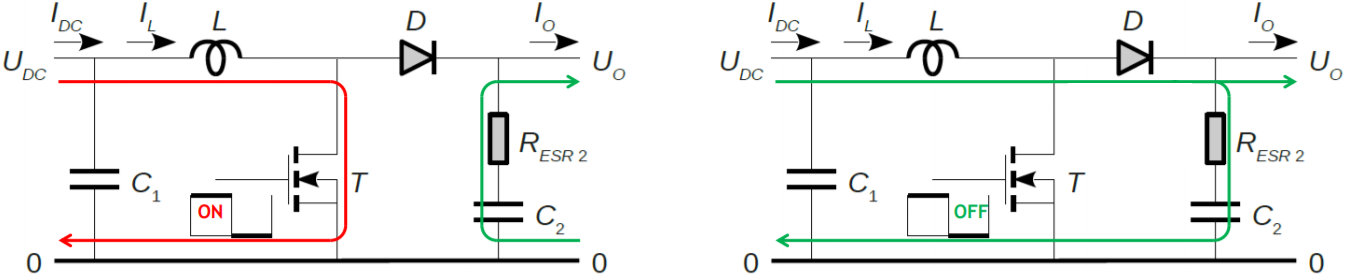
\includegraphics[width=\linewidth]{graphics/dcdc_opkonvertering}
	\caption{Opkonvertering i transistorens to tilstande.}
	\label{fig:dcdc_opkonvertering}
\end{figure}

\paragraph{Nedkonvertering}
\begin{itemize}
	\item Ved nedkonvetering er der byttet rundt på MOSFET, diode og
	spole.
	\item Først når MOSFET’en er slukket løber der ingen strøm i kredsløbet.
	\item Når MOSFET’en tændes begynder strømmen langsomt at stige i spolen, det skaber et modsatrettet spændingsfald. Dette gør at $U_O < U_{DC}$.
	\item Imens strømmen stiger i spolen opbygger den et magnetisk felt.
	\item Når MOSFET’en slukkes vil spolen blive ved med at levere strøm, som opretholder udgangsspændingen.
\end{itemize}

\begin{figure} [H]
	\centering
	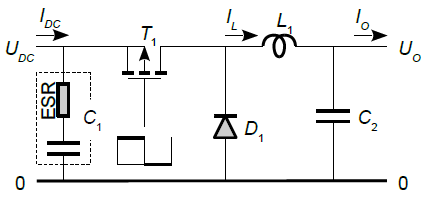
\includegraphics[width=0.6\linewidth]{graphics/nedkonvertering}
	\caption{Nedkonvetering.}
	\label{fig:nedkonvertering}
\end{figure}

\begin{figure} [H]
	\centering
	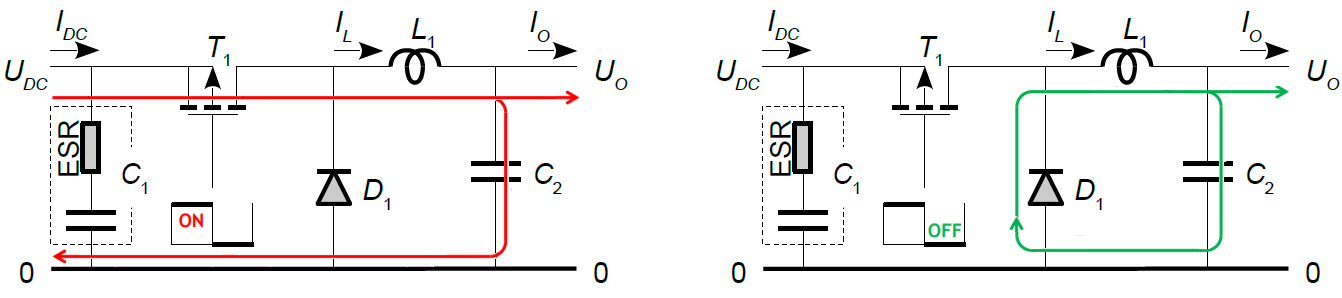
\includegraphics[width=\linewidth]{graphics/dcdc_nedkonvertering}
	\caption{Nedkonvertering i transistorens to tilstande.}
	\label{fig:dcdc_nedkonvertering}
\end{figure}

\newpage 
\section{Operationsforstærkeren}
En OpAmp kan beskrives ved et differentielt indgangstrin der omsætter en spænding til en strøm ved transkonduktansen $g_m$ og en strømforstærker $\beta$ der danner en spænding over $R_C$.

\begin{figure} [H]
	\centering
	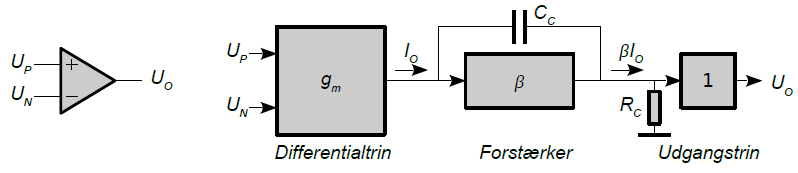
\includegraphics[width=\linewidth]{graphics/opamp_trin}
	\caption{En OpAmp består af et differentielt indgangstrin og en strømforstærker.}
	\label{fig:opamptrin}
\end{figure}

\begin{itemize}
	\item Forstærker forskellen mellems den to indgange, $U_P$ og $U_N$.
	\item Differential-trinnet laver spændingsforskellen om til en strøm $I_O$.
	\item VAS-trinnet forstærker strømmen med $\beta$, som laves til en spænding med $R_C$.
	\item Udgangstrinnet er en unity gain buffer, så udgangen af VAS-trinnet ikke belastes af eksternt load.
	\item Kondensatoren $C_C$ skaber en dominerende pol, der gør OpAmp’en stabil.
	\item DC gain: $A_{DC} = g_m \beta R_C$
	\item AC gain: $A_{OL} = \dfrac{g_m}{\omega C_C}$
\end{itemize}

\subsection{Opbygning og DC forhold}
\begin{itemize}
	\item Trin 1 - laver spændingsdifferens om til en strøm $I_O$ - en transkonduktans blok.
	\item Trin 2 - Forstærker strøm og omsætter til spænding - VAS (Voltage Application Stage).
	\item Trin 3 - Beskytter $R_C$ mod belastningen $R_L$ - omsætter fra mA niveau til A niveau.
\end{itemize}

\begin{figure} [H]
	\centering
	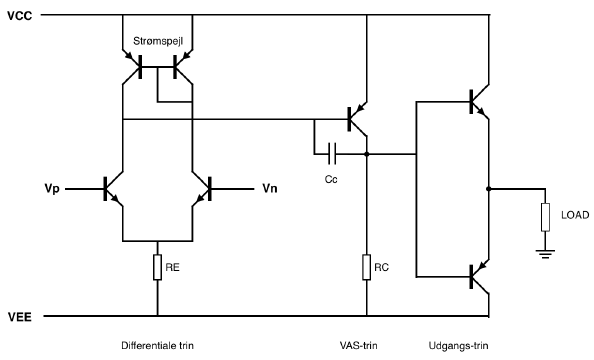
\includegraphics[width=0.85\linewidth]{graphics/opamp}
	\caption{Generelt OpAmp kredsløb.}
	\label{fig:opamp}
\end{figure}
\newpage 
\paragraph{Differentialtrin} benytter to transistorer med fælles emitter, en såkaldt differentielkobling. En strømkilde driver en fast strøm $I_E$ i den fælles emitter. De to transistorer tvinges derfor til at dele strømmen mellem sig. 

\begin{itemize}
	\item Når der ikke er nogen spændingsforskel mellem $U_P$ og $U_N$ vil strømmen i de to transistorer være fordelt 50/50.
	\item Hæves spændingsdifferensen vil T1 trække mere strøm og T2 må så nøjes med en mindre strøm da $I_E$ er konstant. 
	\begin{itemize}
		\item Hvis $U_P$ hæves relativ til $U_N$ vil $I_1$ stige.
	\end{itemize}
\end{itemize} 

\begin{figure} [H]
	\centering
	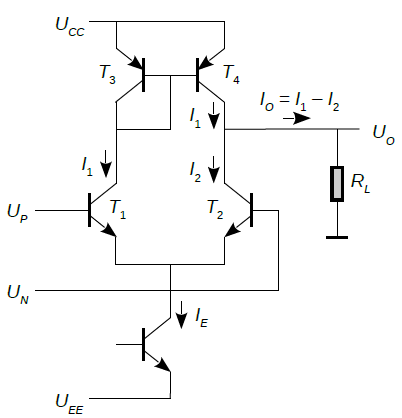
\includegraphics[width=0.3\linewidth]{graphics/differentialtrin}
	\caption{Differentialtrin.}
	\label{fig:differentialtrin}
\end{figure}
	
\paragraph{Strømspejl} udnytter transistorernes ens karakteristik til at indstille strømmen i $I_2$ som er identisk med den strøm $I_1$ det eksterne kredsløb driver i T1.
\begin{itemize}
	\item Differensen mellem de to strømme fra differentialtrinnet dannes af et strømspejl.
	\item Strømmen $I_1$ vil føre til en tilsvarende strøm $I_2$.
	\item Der løber en lille basis-strøm, som i praksis vil føre til en fejl i $I_2$.
\end{itemize}

\begin{figure} [H]
	\centering
	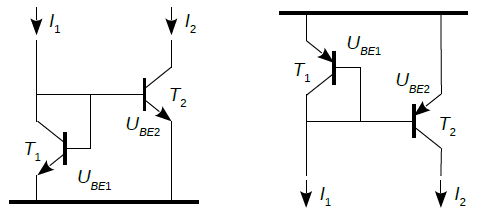
\includegraphics[width=0.6\linewidth]{graphics/currentmirror}
	\caption{Strømspejl.}
	\label{fig:currentmirror1}
\end{figure}

\newpage
\subsubsection{Trin 1: Differentialforstærker}
\begin{itemize}
	\item Kombinerer differentialetrinnet, strømspejlet og strømkilden.
	\item På grund af strømspejlet ved T3 og T4 vil differensen mellem $I_1$ og $I_2$ give en strøm $I_O$ i udgangen.
	\item Der er en øvre grænse for den strøm der kan løbe i udgangen. Det er ikke muligt at få en udgangsstrøm $I_O$ på mere end $I_E$ uanset spændingsdifferensen.
	\item Forholdet fra spændingsforskel til udgangsstrøm kaldes transkonduktansen $g_m$.
	\begin{itemize}
		\item Afhænger af emitterstrømmen fra strømkilden og temperaturspændingen $U_T$.
	\end{itemize} 
\end{itemize}

\begin{equation} 
I_o = g_m(U_P-U_N)
\end{equation}

\begin{equation} 
U_T = \frac{k T}{q_0} \approx \SI{26}{\milli\volt}
\end{equation}

\begin{equation} 
g_m = \frac{I_E}{2nU_T}
\end{equation}

\begin{figure} [H]
	\centering
	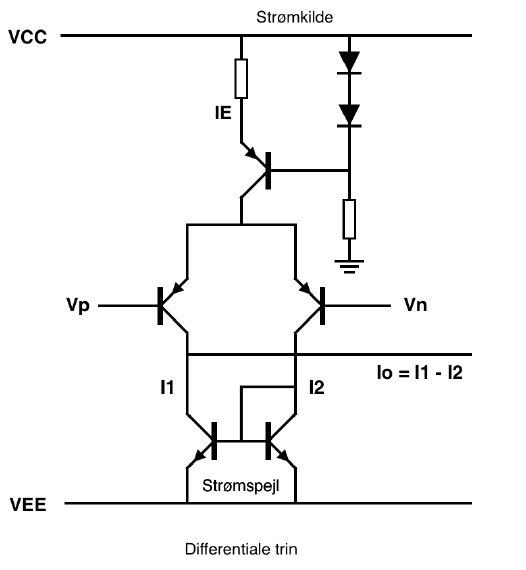
\includegraphics[width=0.7\linewidth]{graphics/differentialtrin_fors}
	\caption{Differentialforstærkertrinnet.}
	\label{fig:differentialforstærker}
\end{figure}



\newpage 
\subsubsection{Trin 2: VAS - Voltage Amplification Stage} 
Transistorens strømforstærkning $\beta$ forstærker differentialtrinnets udgangsstrøm. Denne strøm bliver ledet gennem en modstand, $R_C$, som laver det om til en strøm. 

\begin{figure} [H]
	\centering
	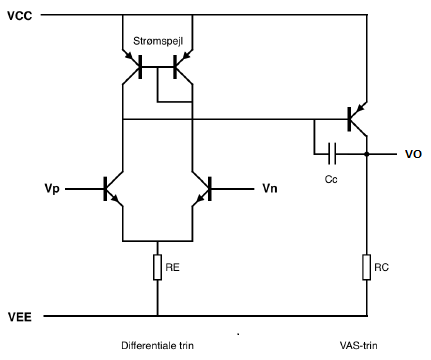
\includegraphics[width=0.7\linewidth]{graphics/vas}
	\caption{Trans-resistans forstærker (VAS).}
	\label{fig:VAS_forstærker}
\end{figure}

I en integreret forstærker benyttes ofte flere transistorer til at forøge den resulterende strømforstærkning mens en effektforstærker oftest nøjes med en enkelt transistor da der ikke er behov for den ekstremt høje forstærkning ved DC. 

\begin{itemize}
	\item Strømmen fra differentialforstærkertrinnet forstærkes op med strømforstærkning $\beta_5$ i T5.
	\item Strømmen ledes gennem $R_C$ der omsætter til en spænding.
	\item DC forstærkningen er givet af transkonduktansen $g_m$, forstærkerens $\beta_5$ for T5 og modstanden $R_C$.
\end{itemize}

\begin{equation} 
A_{DC} = g_m \beta R_C
\end{equation}

\begin{itemize}
	\item Kondensatoren $C_C$ skaber en dominerende pol ved $f_0$, som sikrer stabilitet.
\end{itemize}

\begin{equation} 
f_0 = \dfrac{1}{2 \pi \beta R_C C_C}
\end{equation}
\\
Den dominerende pol giver stabilitet, men begrænser også hvor hurtigt udgangen kan flyttes. Hvis værdien forsøges overskredet bliver signalet forvrænget.

\begin{itemize}
	\item Slew-raten (SR) begrænses af kondensatoren og strømmen $I_E$.
\end{itemize}

\begin{equation} 
SR = \dfrac{I_E}{C_C}
\end{equation}

\subsection{AC forhold og stabilitet}
\begin{itemize}
	\item En operationsforstærker har mindst to poler.
	\item En tilbagekoblet operationsforstærker skal have en dominerende pol for stabilitet.
	\item Ved tilbagekobling giver det en overføringsfunktion af mindst andet orden og det kan give problemer med stabilitet.
	\item For at gardere sig kan man vælge den dominerende pol $f_0$ så lavt at systemet bliver ubetinget stabilt.
\end{itemize}

\begin{equation} 
f_0  \leq \frac{f_h}{4\,A_{DC}}
\end{equation}

\begin{equation} 
C_C  = \frac{1}{2\pi \beta f_0 R_C}
\end{equation}


\begin{itemize}
	\item Miller transformation udføres for at finde modstande og kapaciteter, der resulterer i poler.
\end{itemize}

\begin{equation} 
g_{m5} = \frac{I_C}{U_T}
\end{equation}

\begin{equation} 
A = g_{m5} R_C
\end{equation}

\begin{equation} 
r_{\pi 5} = \frac{\beta_5}{g_{m5}}
\end{equation}

\begin{equation} 
C_{\si{\micro}5} = C_{MO5}
\end{equation}

\begin{equation} 
C_{MI5} = (1+A)C_{MO5}
\end{equation}

\begin{itemize}
	\item Polen ved ind- og udgangen findes.
\end{itemize}

\begin{equation} 
f_1 = \dfrac{1}{2\pi \, r_{\pi} (C_{\pi} + C_{MI5})}
\end{equation}

\begin{equation} 
f_2 = \dfrac{1}{2\pi \, r_C \, C_{MO5}}
\end{equation}

\begin{itemize}
	\item Den nye dominerende pol findes ud fra den høje pol.
\end{itemize}

\begin{equation} 
f_0  \leq \frac{f_h}{4\,A_{DC}}
\end{equation}

\begin{itemize}
	\item Kompenseringskondensatoren kan nu vælges.
\end{itemize}

\begin{equation} 
C_C  = \frac{1}{2\pi \beta f_0 R_C}
\end{equation}
\\

Polen mellem differentialtrinnets T1 til T4 og VAS-trinnets T5 bliver normalt ofret ved at inkludere $C_C$ der sænker polens frekvens så den udgør operationsforstærkerens dominerende pol. \\

Der er en fordel ved valget idet kapaciteten $C_{\si{\micro}}$ fra kollektor til basis ved T5 bliver stort set uden betydning. 
Det er væsentligt fordi operationsforstærkerens egenskaber ved høje frekvenser defineres af netop denne kapacitet.
Det betyder at kondensatoren er aktiv i hele frekvensområdet for den dominerende pol. 
Transistorens kapacitet $C_{\si{\micro}}$ er spændingsafhængig og vil derfor introducere harmonisk forvrængning, men ved at parallelkoble $C_{\si{\micro}}$ med en stabil kapacitet $C_C$ kan forvrængningen sænkes. \\
 
Et design af en operationsforstærker bliver et kompromis mellem at opnå en hurtig forstærker, altså en stor slew rate, og stabilitet, altså en lav værdi af GBP. 

\subsubsection{Trin 3: Udgangstrin} 
Udgangstrinnets opgave er at kunne levere (eller optage) en stor strøm til (fra) belastningen $R_L$ samt at isolere det relativt høje impedansniveau ved kollektor af T5 fra belastningens varierende værdi.\\

Modstanden $R_C$ er faktor i udtrykket for åben-sløjfe forstærkningen $A_{OL}$ og ønskes derfor til en høj værdi. Det giver så til gengæld en pol ved udgangen af forstærkertrinnet.

\begin{itemize}
	\item Udgangstrinnet adskiller VAS trinnets $R_C$ fra udgangsbelastningen.
	\item Kan gøres med et par emitterfølgere - eventuelt to dobbelt emitter-følgere, der øger dens evne til at levere strøm.
\end{itemize}

\begin{figure} [H]
	\centering
	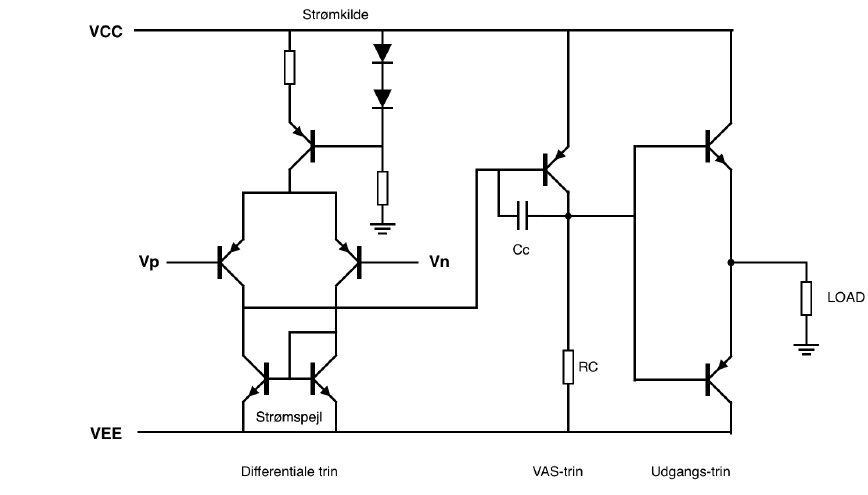
\includegraphics[width=0.85\linewidth]{graphics/udgangstrin}
	\caption{Udgangstrin.}
	\label{fig:udgangstrin}
\end{figure}

\subsection{Offset-fejl og støj}
Se side 280 i Analogteknik.
\newpage
\section{Dioden}
Diodens egenskab er PN overgangen der kun tillader en elektrisk strøm at løbe i én retning. 
I modsatte retning løber en ubetydelig strøm indtil spændingen over dioden bliver så stor at PN overgangen bryder sammen og strømmen vokser hurtigt.

\begin{itemize}
	\item Dioden er afbrudt når anodens spænding er lavere end katodens spænding.
	\item Dioden repræsenteres af en spændingsforskel på 0,7 V når anodens spænding er højere end katoden og der løber en strøm.
\end{itemize}

\begin{itemize}
	\item I det ledende område er strømmen en eksponentiel funktion af diodens spænding.
	\begin{equation}
	I_F = I_s \exp \left(\dfrac{U_F}{n U_T}\right)
	\end{equation}
	\item I det spærrende område er strømmen meget lille, men varierer nu eksponentielt med temperaturen. 
	\begin{equation}
	I_R = I_{R0} 2^{(T-T_0)/\Delta{T}}
	\end{equation}
	\item I zener området vil diodens strøm vokse voldsomt når spændingen over dioden overskrider en grænse hvorved PN overgangen bryder sammen.
	\item Relationen er eksponentiel og strømmen vokser en dekade
	ved en ændring af spændingen over dioden på cirka 60 mV for n = 1. Relationen vil almindeligvis holde over et område på seks dekader fra 10 nA til 10 mA for småsignaldioder.
\end{itemize}

\begin{figure} [H]
	\centering
	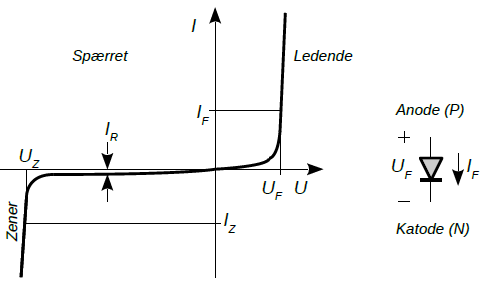
\includegraphics[width=0.85\linewidth]{graphics/I-U_karakteristik}
	\caption{Diodens karakteristik I(U).}
	\label{fig:I-U_karakteristik}
\end{figure}


\subsection{PN overgangen}
Dioden består af et P-lag og et N-lag, med henholdsvis et underskud og et overskud af elektroner.
\begin{itemize}
	\item Diodens N halvleder har et overskud af frie elektroner.
	\item Diodens P halvleder har et overskud af flytbare huller. 
	\item Diffusionen af elektroner danner et elektrisk felt som modvirker diffusionen. Elektronerne fra N-laget diffunderer mod P-laget.
	\item En ekstern spændingskilde kan ændre på det elektriske felt og derved styre strømmen i dioden.
\end{itemize}

\begin{figure} [H]
	\centering
	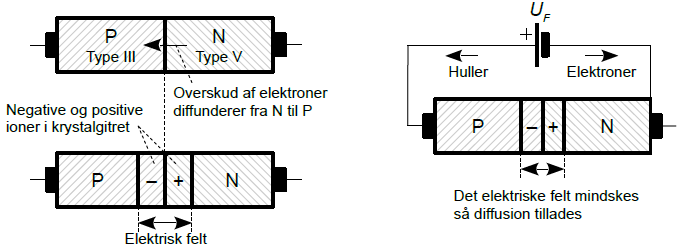
\includegraphics[width=\linewidth]{graphics/PN_overgang}
	\caption{PN overgangen.}
	\label{fig:pnovergang}
\end{figure}

Hvis der påtrykkes en ekstern spænding med plus ved P og minus ved N vil det tilføre frie elektroner til N halvlederen som mindsker det elektriske felt.
Derved kan elektroner diffundere gennem PN overgangen og rekombinere med hullerne i P halvlederen. \textbf{Der løber en elektrisk strøm i dioden}. \\

Hvis det eksterne batteri vendes om vil det elektriske felt øges og blokere for en strøm. \textbf{Dioden spærrer.}


\subsection{Modeller - AC/DC}
\paragraph{DC modellen} for dioden har en DC modstandsværdi, $R_D$, som resulterer i et større målt spændingsfald, $U_D$, i lederetningen ved en given strøm $I_F$.

\begin{equation}
U_D = U_F + R_D I_F
\end{equation}

\begin{itemize}
	\item Seriemodstanden skyldes ledningsevnen af halvlederens materiale.
	\item Modstanden $R_D$ er ikke en konstant værdi.
\end{itemize}

\begin{figure} [H]
	\centering
	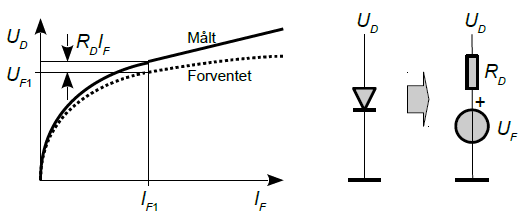
\includegraphics[width=0.9\linewidth]{graphics/DC_diode}
	\caption{Diodens seriemodstand ved DC.}
	\label{fig:DC_diode}
\end{figure}

\newpage
\paragraph{AC modellen} for dioden hvor seriemodstanden er ubetydelig, kan dioden ses som en strømstyret modstand. 
Modstanden falder ved højere strømme.

\begin{equation}
r_D = \dfrac{U_T}{I_F}
\end{equation}

\begin{figure} [H]
	\centering
	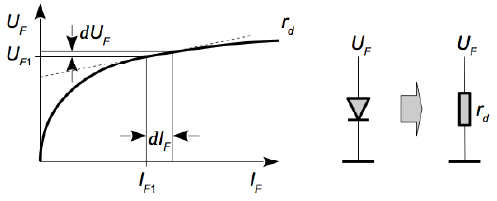
\includegraphics[width=0.8\linewidth]{graphics/ACdiode}
	\caption{Diodens seriemodstand ved AC.}
	\label{fig:AC_diode}
\end{figure}

\subsection{Anvendelser}
\paragraph{Ensretning} Halvbølge ensretning af et vekselsignal giver en pulserende jævnstrøm.

\begin{itemize}
	\item Hvis indgangssignalet er positivt vil udgangen følge med indgangssignalet i den positive halvperiode dog med en forskel på cirka \SI{0,7}{\volt}.
	\item Hvis indgangssignalet er negativt vil dioden spære da der kun kan løbe strøm i diodens lederetning.
\end{itemize}

\begin{figure} [H]
	\centering
	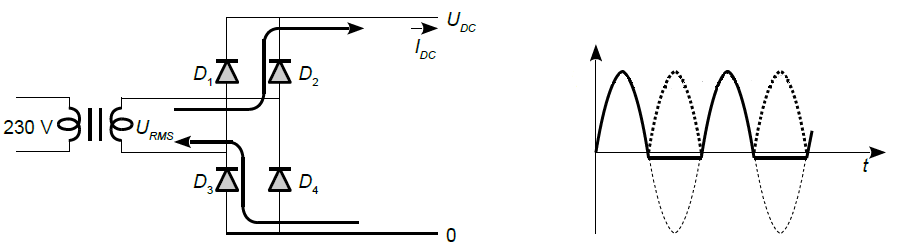
\includegraphics[width=\linewidth]{graphics/ensretning}
	\caption{Halvbølge ensretning af et vekselsignal.}
	\label{fig:ensretning}
\end{figure}

\paragraph{Beskyttelseskredsløb} Dioden kan beskytte en følsom indgang imod overspænding.

\begin{figure} [H]
	\centering
	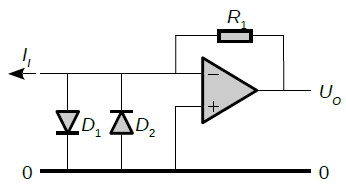
\includegraphics[width=0.5\linewidth]{graphics/diodebeskyt}
	\caption{Beskytning af en følsom indgang imod overspænding.}
	\label{fig:diodebeskyt}
\end{figure}

\newpage
\section{Transistoren: DC}

\subsection{DC model}
Der er to modeller for hvordan transistorens kollektorstrøm styres.
\begin{figure} [H]
	\centering
	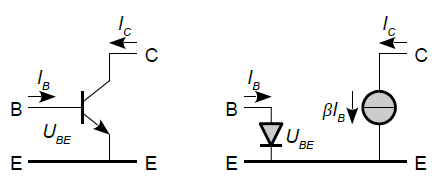
\includegraphics[width=0.6\linewidth]{graphics/transistor_DCmodel}
	\caption{Transistorens strøm er styret af base-emitter spændingen eller basisstrømmen.}
	\label{fig:transistor_DCmodel}
\end{figure}

\textbf{DC model 1 – Spændingsstyret}
\begin{itemize}
	\item Spændingen over transistorens base-emitter junction, $U_{BE}$, styrer kollektorstrømmen $I_C$.
	\item Basisstrømmen er ${\beta}$ gange mindre end kollektorstrømmen.
\end{itemize}

\begin{equation}
I_C = I_S \exp \dfrac{U_{BE}}{n U_T}
\end{equation}

\begin{equation}
I_B = \dfrac{I_C}{\beta}
\end{equation}

\textbf{DC model 2 – Strømstyret}
\begin{itemize}
	\item Basisstrømmen $I_B$ styrer kollektorstrømmen $I_C$.
	\item Strømforstærkningen ${\beta}$ er typisk mellem 100 og 1000 for småsignal transistorer.
	\item Effektransistorer forstærker 10 til 100 gange.
\end{itemize}
 
\begin{equation}
I_C = I_B {\beta}
\end{equation}

\begin{equation}
U_{BE} = n U_T \ln \dfrac{I_C}{I_S}
\end{equation}

\subsection{Forskellige typer (BJT, FET)}

\paragraph{BJT} er en bipolar transistor som fremstilles ud fra en diode ved at tilføje endnu et lag halvleder. 

\begin{itemize}
	\item Der er to måder PN overgangene kan arrangeres på: NPN og PNP.
	\item De er komplementære transistorer.
	\item Meget ens, men lidt større diode spændingsfald ved en PNP.
\end{itemize}

Ved NPN tilføres et ekstra N lag mod diodens anode hvorved elektronerne kan løbe videre i ledningsbåndet til det nye N lag der kaldes for kollektor.\\
 
Hvis bredden af P laget er væsentlig mindre end rekombinationslængden vil hovedparten af elektronerne fortsætte fra emitter til kollektor.
De elektroner der rekombinerer i basis laget udgør transistorens basisstrøm. 

\begin{figure} [H]
	\centering
	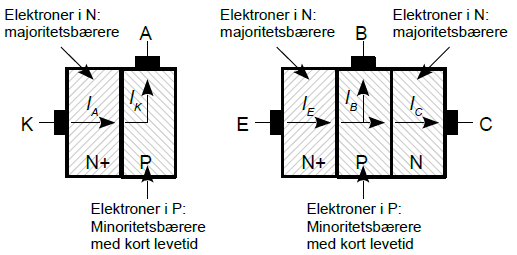
\includegraphics[width=0.7\linewidth]{graphics/bjt}
	\caption{En NPN opbygning med emitter (N+), basis (P) og kollektor (N).}
	\label{fig:bjt}
\end{figure}

\begin{figure} [H]
	\centering
	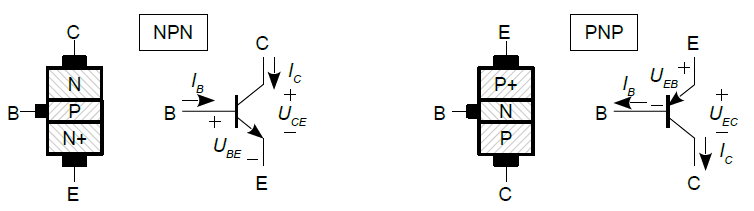
\includegraphics[width=\linewidth]{graphics/transistor}
	\caption{NPN og PNP transistor.}
	\label{fig:transistor}
\end{figure}

\paragraph{JFET} er en betegnelse for junction field effect transistor. 
Den har tre elektroder der benævnes \textit{gate} for styreelektroden, \textit{source} for strømkilden og \textit{drain} for opsamling af
elektronerne. 

Styreelektroden gate er forbundet til kanalen mellem drain og source via en spærrende diode. 
Med en negativ spænding på gate i forhold til source vil det elektriske felt frastøde elektroner i nærheden af dioden. 
Modstanden af kanalen er givet ved antallet af frie elektroner.
Hvis kanalen indsnævres ved det elektriske felt fra gate vil der være færre elektroner og derved en højere modstandsværdi mellem source og drain.

\begin{itemize}
	\item Transistoren er åben uden spænding på gate $V_{GS}=0$. Kaldes Depletion mode.
	\item En negativ gate-source spænding vil begynde at begrænse drain-strømmen $I_D$ \newline (modsat for en P kanal JFET).
	\item Transistoren er helt spærende ved den negative pinch off spænding: $V_P$.
\end{itemize}

\begin{figure} [H]
	\centering
	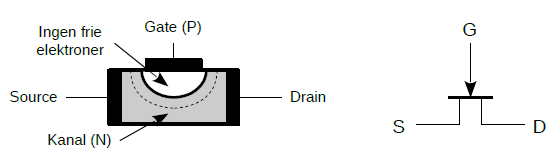
\includegraphics[width=0.8\linewidth]{graphics/jfet}
	\caption{JFET transistor.}
	\label{fig:jfet}
\end{figure}

Kanalen mellem source og drain er i mange tilfælde symmetrisk og de to elektroder kan da ombyttes. Hvis det ikke er tilfældet tegnes pilen nærmest ved source.


\paragraph{MOSFET} er betegnelsen for en metal-oxide silicon field-effect transistor. 
Gate-elektroden er opbygget som et metallag med et tyndt lag siliciumoxyd som isolator mellem gate og kanal.

\begin{itemize}
	\item Mosfetten spærer for strøm når gate-spændingen $V_{GS} < V_{GS (th)}$. Kaldes Enhancement mode.
	\item Der kan løbe strøm i drain når gaten lades op (det tager tid, som en kondensator).
	\item Gate kapaciteten begrænser hvor hurtigt den kan tænde/slukke.
\end{itemize}

\begin{figure} [H]
	\centering
	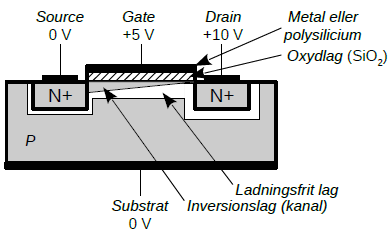
\includegraphics[width=0.5\linewidth]{graphics/mosfet}
	\caption{MOSFET transistor opbygning.}
	\label{fig:mosfet}
\end{figure}

\begin{figure} [H]
	\centering
	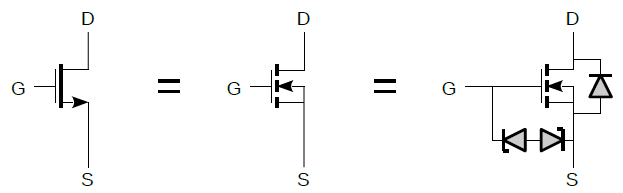
\includegraphics[width=0.8\linewidth]{graphics/mosfet_symbol}
	\caption{MOSFET transistor symbol.}
	\label{fig:mosfet_symbol}
\end{figure}

\subsection{Anvendelser}
\paragraph{Diodekobling} En diode-koblet transistor opfører sig fuldstændig som en diode.
\begin{itemize}
	\item Ved at korslutte basis og kollektor bliver transistoren en diode.
	\item Hyppigt brugt i IC design.
	\item Anvendes i strømspejlet.
\end{itemize}

\begin{figure} [H]
	\centering
	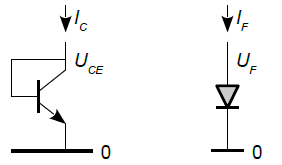
\includegraphics[width=0.5\linewidth]{graphics/diodekobling}
	\caption{Transistoren kan benyttes som diode.}
	\label{fig:diodekobling}
\end{figure}

\paragraph{Strømspejl}
En strøm $I_1$ i transistor $T_1$ vil give en tilsvarende strøm $I_2$ i transistor $T_2$ så det er muligt at bruge strømmen i ét kredsløb til at styre en strøm i et andet.
\begin{itemize}
	\item Strømmen $I_1$ vil føre til en tilsvarende strøm $I_2$.
	\item Der løber en lille basis-strøm, som i praksis vil føre til en fejl i $I_2$.
\end{itemize}

\begin{figure} [H]
	\centering
	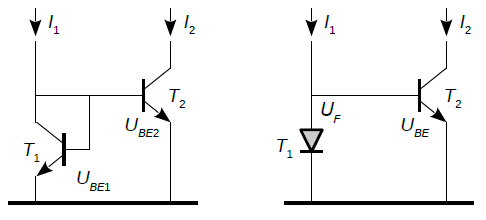
\includegraphics[width=0.8\linewidth]{graphics/diodekobling1}
	\caption{Strømspejl.}
	\label{fig:currentmirror}
\end{figure}

\begin{equation} 
U_F = n U_T \ln{\left(\frac{I_S}{I_1}\right)}
\end{equation}

\begin{equation} 
U_{BE} = U_F
\end{equation}

\begin{equation} 
I_2 = I_S \exp{\left(\frac{U_{BE}}{n U_T}\right)}
\end{equation}

\begin{equation} 
I_2 = I_S \exp{\left(\frac{n U_T \ln{\left(\frac{I_S}{I_1}\right)}}{n U_T}\right)}
\end{equation}

\newpage
\section{Transistoren: AC}
\subsection{AC model}
\paragraph{Linearitet} kan for en transistor opnås ved at holde signalniveauet lavt. Arbejdspunktet må ikke komme tæt på $I_C = \SI{0}{\milli\ampere}$ og må kun svinge få mV omkring dette arbejdspunkt. 

\begin{itemize}
	\item Det antages at transistoren er ved et fornuftigt DC-arbejdspunkt. AC-spændingerne varierer omkring det faste arbejdspunkt.
	\item Det antages at kredsløbet er lineært, som tillader superposition og dermed	adskillelse mellem DC og AC-analysen (småsignalmodel).
	\item DC-arbejdspunktet angives med $I_B$, $I_C$ og $U_BE$.
	\item AC-værdierne angives med $i_B$, $i_C$ og $u_BE$.
\end{itemize}

Strømmen i kollektor $i_C$ variererer proportionalt med $u_{BE}$ ved svagt signal.

\begin{equation} 
i_C = g_m u_{BE}
\end{equation}

\begin{equation} 
i_C = \dfrac{I_C}{n U_T} u_{BE}
\end{equation}

\begin{figure} [H]
	\centering
	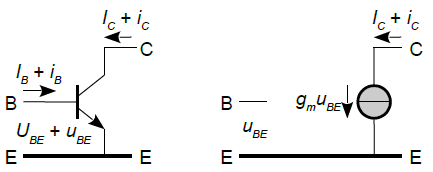
\includegraphics[width=0.75\linewidth]{graphics/ACmodel}
	\caption{Simpel AC model.}
	\label{fig:ACmodel}
\end{figure}

DC arbejdspunktet $I_C$ giver fundamentet for AC modellens vigtigste parameter: transkonduktansen.

\paragraph{Transkonduktansen} er proportionaliteten mellem småsignals-kollektorstrømmen $i_C$ som funktion af spændingen $u_{BE}$. 
Den beskriver ledningsevnen i siemens (S).\\

For at finde et arbejdspunkt hvor det er muligt at lave denne småsignals overførelse, laves en DC analyse hvor $I_C$  og $U_{BE}$ bestemmes. Ud fra disse kan transkonduktansen findes som:

\begin{equation} 
g_m = \dfrac{I_C}{U_T}
\end{equation}

\newpage
\paragraph{Miller-transformation} benyttes for at adskille transistorens ind- og udgangsporte. Ved et eksempel med en mikrofon forstærker vises Miller-transformationen. Først oversættes kredsløbet til en AC model.
\begin{figure} [H]
	\centering
	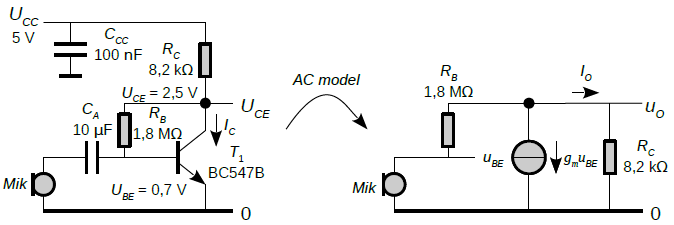
\includegraphics[width=0.8\linewidth]{graphics/mikrofon}
	\caption{Mikrofonforstærker oversat til en AC model.}
	\label{fig:mikrofonforstærker}
\end{figure}

Forstærkningen bestemmes af transkonduktansen og modstanden $R_C$.
\begin{equation} 
A = \dfrac{u_o}{u_{BE}} = -g_m R_C
\end{equation}

Transistoren har en intern kapacitet $C_{\si{\micro}}$ i den spærrende diode i kollektor-basis og den begrænser den opnåelige båndbredde.

\begin{itemize}
	\item $C_{\si{\micro}}$ transformeres fra ud- til indgangen ved at gange med forstærkningen A + 1.
	\begin{itemize}
		\item Udgangen: $C_{\si{\micro}MO} = C_{\si{\micro}}$
		\item Indgangen: $C_{\si{\micro}MI} = C_{\si{\micro}}(A + 1)$
	\end{itemize}
	\item $R_B$ tranformeres til indgangen ved at dele med $(A + 1)$.
\end{itemize}

\begin{figure} [H]
	\centering
	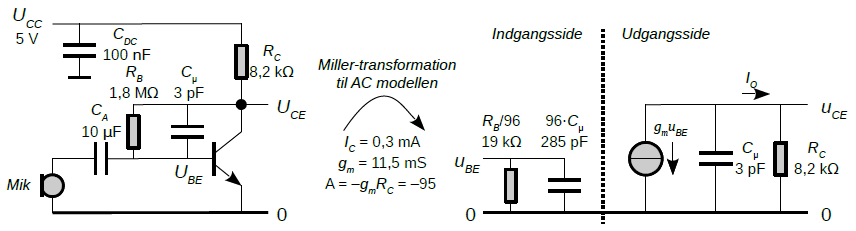
\includegraphics[width=\linewidth]{graphics/millertransformation}
	\caption{Mikrofonforstærker med kapaciteten $C_{\si{\micro}}$ indtegnet.}
	\label{fig:millertransformation}
\end{figure}

\newpage
\subsection{Støj og forvrængning}
Forstærkeren er ikke støjfri da der genereres termisk støj fra modstandene og haglstøj fra strømmene i basis og kollektor.
\begin{itemize}
	\item Termisk støj $e_{nR}$ fra modstandene.
	\begin{itemize}
		\item Signalkildens indre modstand $R_G$.
		\item Basismodstanden $r_x$.
	\end{itemize}
\end{itemize}

Støjbidraget fra den indre modstand $R_G$ og transistorens modstand i basis $r_X$.
\begin{equation} 
e_{nR} = \sqrt{4kT(R_G+r_x)}
\end{equation}

\begin{itemize}
	\item Haglstøj fra strømmene i basis og kollektor.
	\begin{itemize}
		\item Basis $i_{nB} = \sqrt{2 q_0 I_B}$
		\item Kollektor $i_{nC} = \sqrt{2 q_0 I_C}$
	\end{itemize}
\end{itemize}

Støjbidraget fra strømmen $I_B$ i basis som løber gennem $R_G$ og
$r_X$.

\begin{equation} 
e_{nB} = (R_G+r_x)i_{nB}
\end{equation}

Støjbidraget fra strømmen $I_C$ i kollektor som løber gennem den eksterne modstand $R_C$.

\begin{equation} 
e_{nC} = U_T \sqrt{\dfrac{2q_0}{I_C}}
\end{equation}

Samlet indgangsstøj

\begin{equation} 
e_{nTOT} = \sqrt{e_{nR}^2+e_{nB}^2+e_{nC}^2}
\end{equation}

\begin{figure} [H]
	\centering
	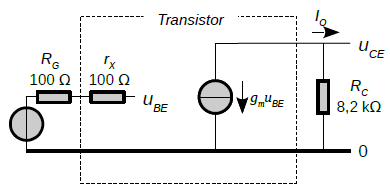
\includegraphics[width=0.5\linewidth]{graphics/stoj}
	\caption{Egenstøj fra transistor.}
	\label{fig:stoj}
\end{figure}

Modstanden $r_x$ kan udregnes udfra transistorens støjtal NF som er opgivet i databladet. NF angiver det antal decibel hvormed transistoren forringer det mulige signal/støj forhold.

\begin{equation} 
r_x = R_G (10^{NF/\SI{10}{\decibel}}-1)
\end{equation}

Transistorens forvrængning kan holdes til \SI{1}{\percent} THD (total harmonic distortion) ved at indgangssignalet varierer med mindre end \SI{1}{\milli\ampere}. \\

Dette skyldes transistorens eksponentielle karakteristik.

\newpage
\subsection{Koblingstyper og deres egenskaber}
\paragraph{Inverterende forstærker} med en forstærkning der teoretisk bør være $-\dfrac{R_B}{R_A}$.\\

Det holder dog ikke i praksis pga. den lave åben-sløjfe forstærkning og indgangsmodstanden ved transistorens basis.

\begin{figure} [H]
	\centering
	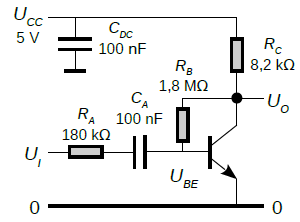
\includegraphics[width=0.4\linewidth]{graphics/inverterende_for}
	\caption{Inverterende forstærker.}
	\label{fig:inverterende_for}
\end{figure}
		



\end{document}